\documentclass[11pt]{amsart}
\usepackage{geometry}                % See geometry.pdf to learn the layout options. There are lots.
\geometry{letterpaper}                   % ... or a4paper or a5paper or ... 
%\geometry{landscape}                % Activate for for rotated page geometry
\usepackage[parfill]{parskip}    % Activate to begin paragraphs with an empty line rather than an indent
\usepackage{graphicx}
\usepackage{amssymb}
\usepackage{epstopdf}  
\usepackage{hyperref}
  \usepackage{color}
  \definecolor{linkcol}{rgb}{0,0,0.4}
  \definecolor{citecol}{rgb}{0.5,0,0}
  \hypersetup
  {
  pdfauthor="Mathieu Guigue", %auteur du document
  %pdftoolbar=false, %barre d'outils non visible 
  pdfmenubar=true, %barre de menu visible
  colorlinks=true, %couleurs sur les liens hypertextes
  pdfpagemode=UseNone, %aucun mode de page
  pdfpagelayout=SinglePage, %ouverture en simple page
  pdffitwindow=true, %pages ouvertes entierement dans toute la fenetre
  linkcolor=linkcol, %couleur des liens hypertextes internes
  citecolor=citecol, %couleur des liens pour les citations
  urlcolor=linkcol %couleur des liens pour les url
  }
\DeclareGraphicsRule{.tif}{png}{.png}{`convert #1 `dirname #1`/`basename #1 .tif`.png}

\newtheorem{tgf}{To-Go-Further}


\title{Report about the assignment}
\author{Mathieu Guigue}
\date{\today}                                           % Activate to display a given date or no date

\begin{document}
\maketitle

\section{Introduction}

\section{Part 1: Data averaging}
\subsection{Time series}

\begin{figure}
    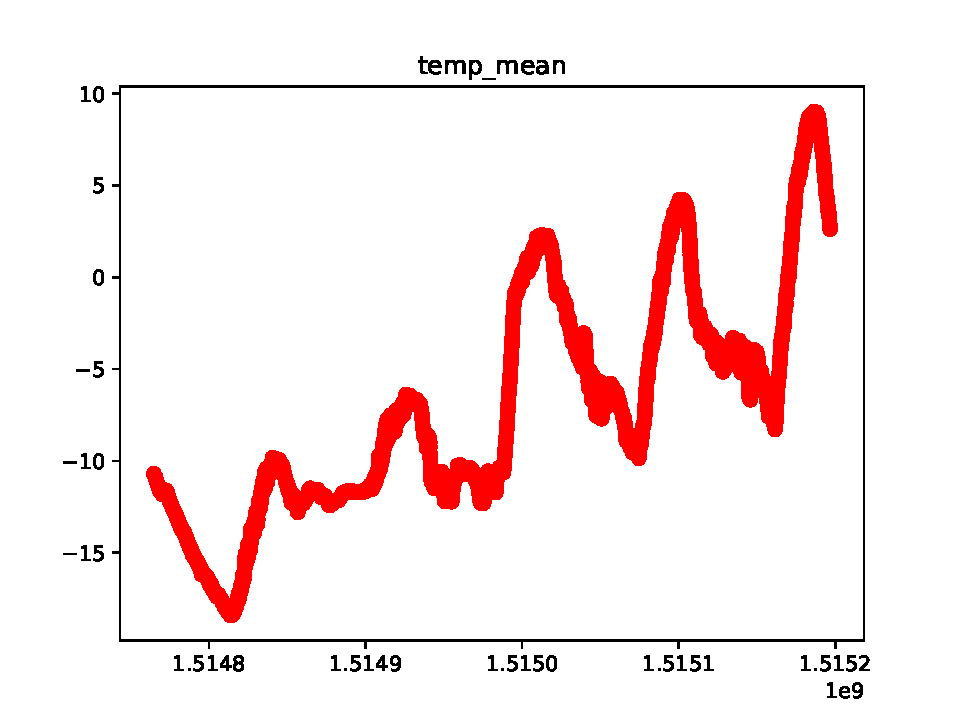
\includegraphics[width=0.45\textwidth]{../plots/temp_mean.pdf}
    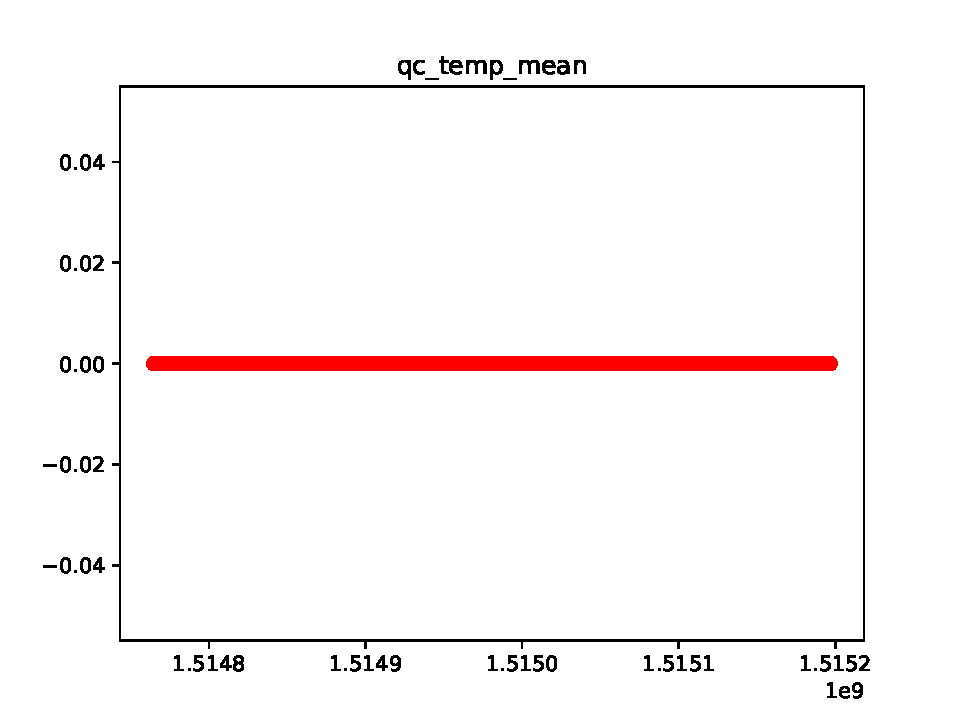
\includegraphics[width=0.45\textwidth]{../plots/qc_temp_mean.pdf}
    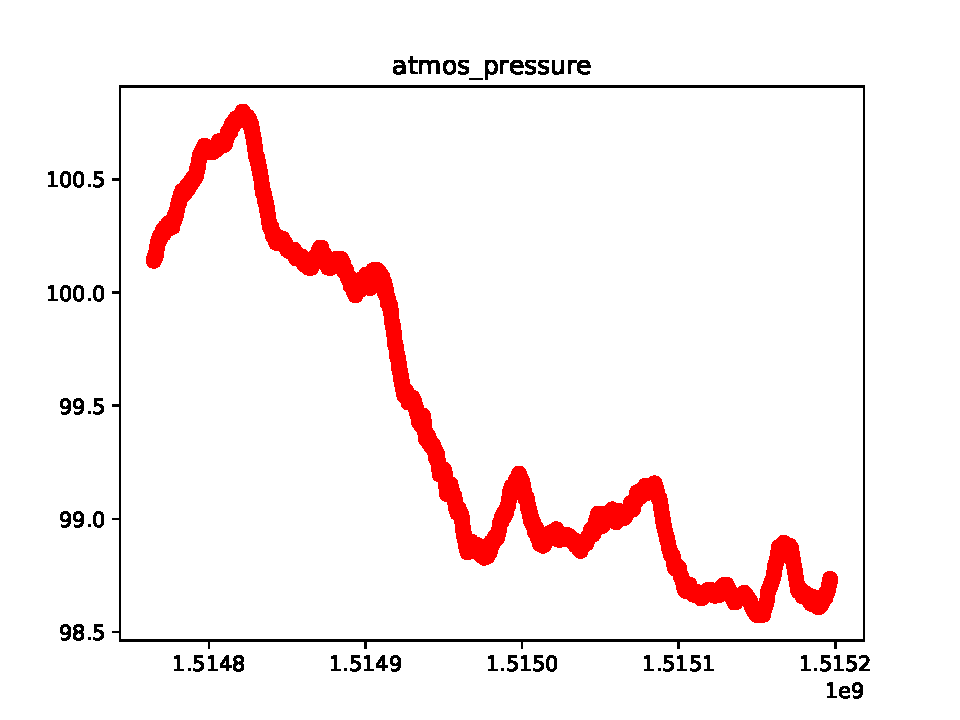
\includegraphics[width=0.45\textwidth]{../plots/atmos_pressure.pdf}
    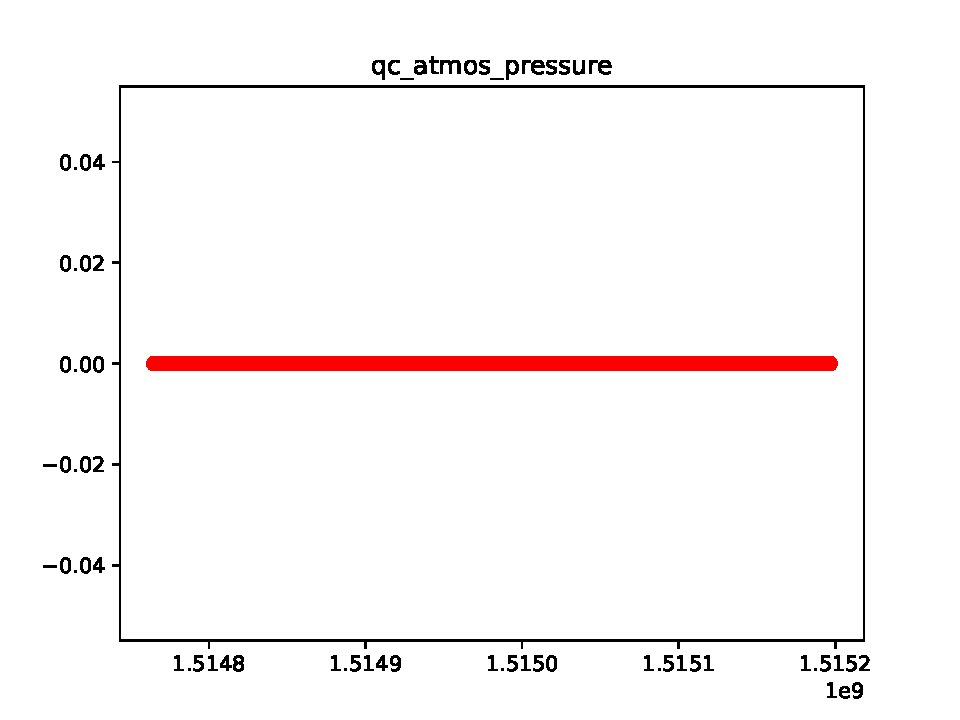
\includegraphics[width=0.45\textwidth]{../plots/qc_atmos_pressure.pdf}
    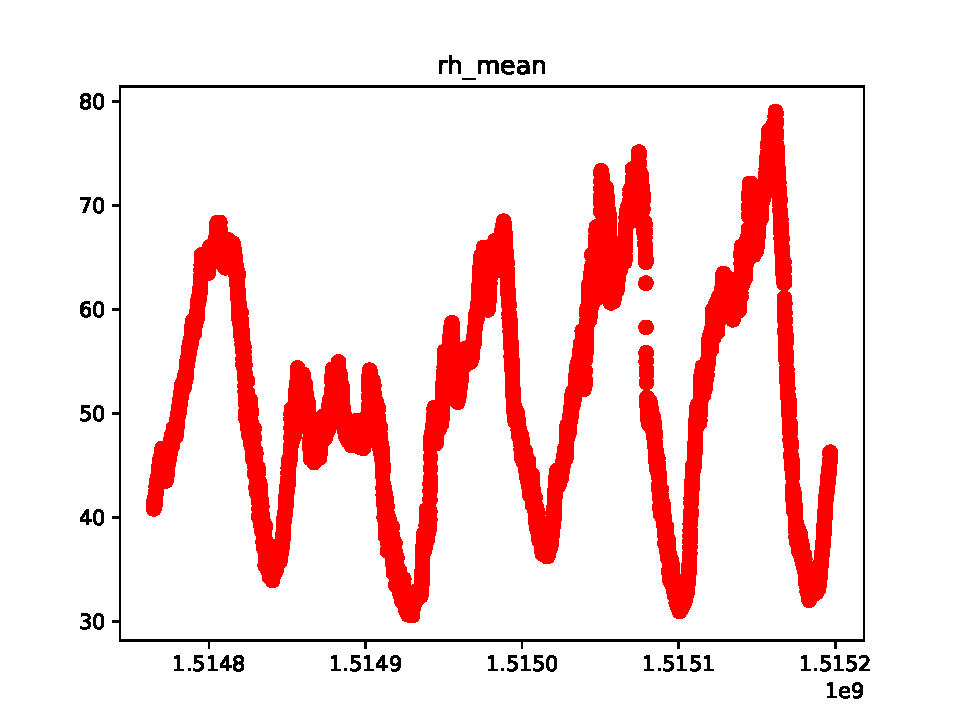
\includegraphics[width=0.45\textwidth]{../plots/rh_mean.pdf}
    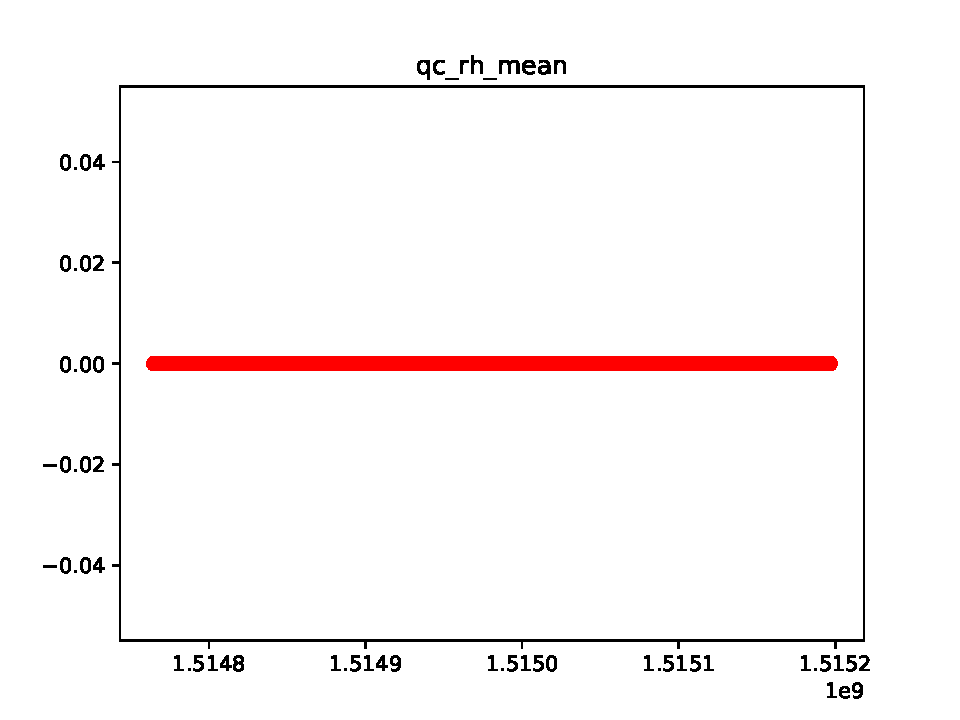
\includegraphics[width=0.45\textwidth]{../plots/qc_rh_mean.pdf}
    \caption{Time series of the mean temperature, mean relative humidity and atmospheric pressure (left) and the associated quality check value (right) as a function of time.}
\end{figure}
%\begin{figure}
%    \caption{Time series of the quality checks for mean temperature, mean relative humidity and atmospheric pressure as a function of time.}
%\end{figure}

Each file corresponds to a day of data, one data point every 60 seconds.
Each day has its own time stamp (number of seconds since midnight) and a hardcoded-modification of the reader function is required to get things working.

\subsection{Estimating the optimal average period}

Using an Allan representation of the data, I can estimate what the typical period where the measurements fluctuations are Gaussian is.
It seems that the value at which non Gaussian fluctuations appear is defined for all three variables to be about 60 samples.
For safety, I will use 50 samples for averaging.

\begin{figure}
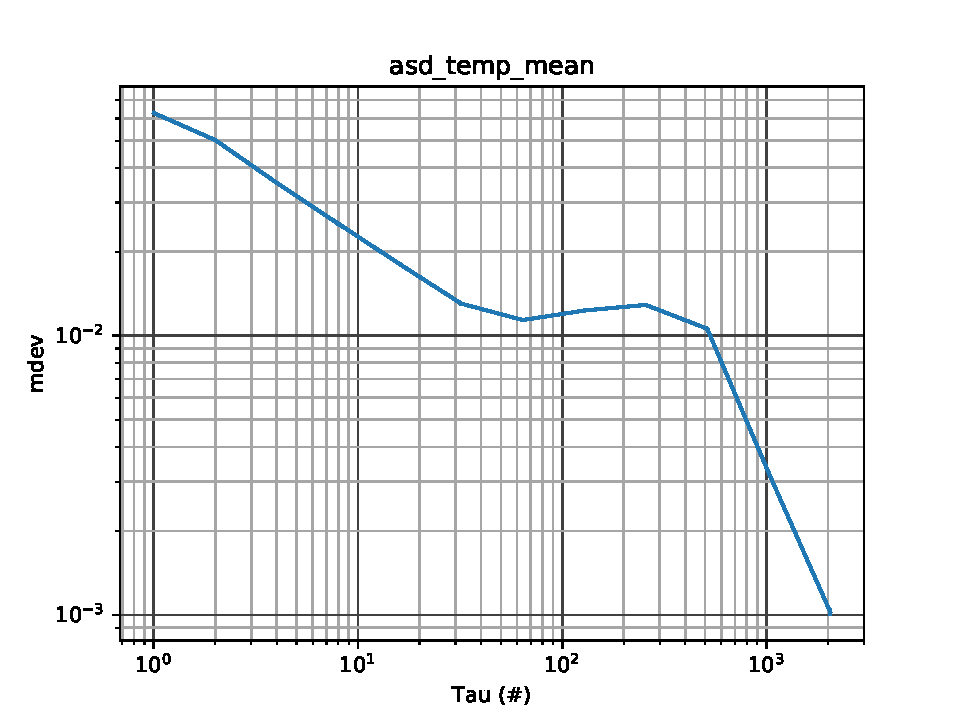
\includegraphics[width=0.6\textwidth]{../plots/asd_temp_mean.pdf}
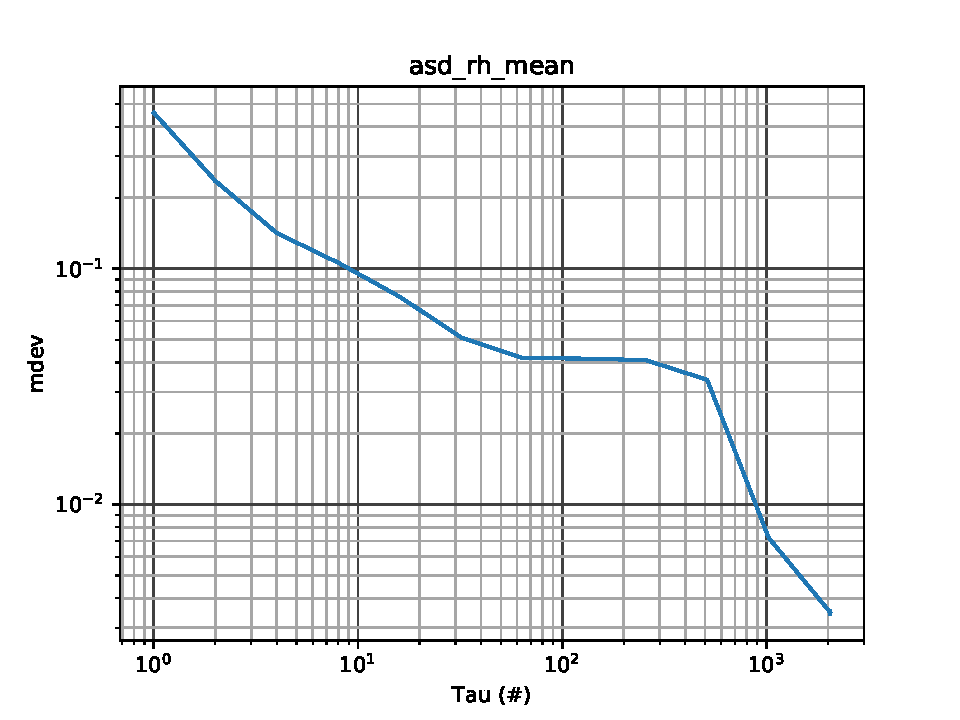
\includegraphics[width=0.6\textwidth]{../plots/asd_rh_mean.pdf}
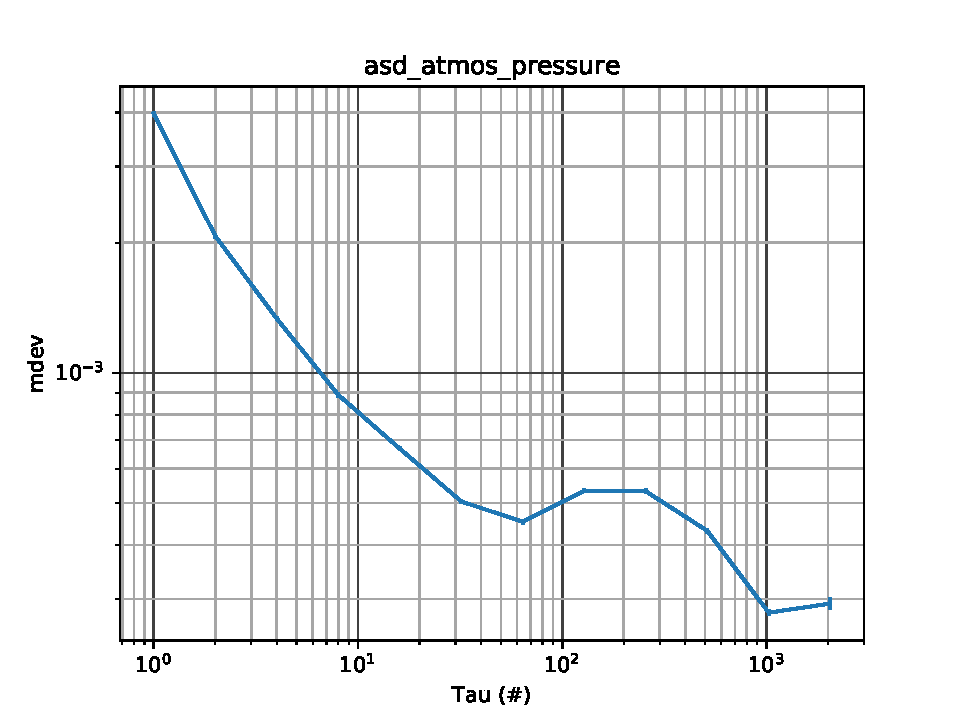
\includegraphics[width=0.6\textwidth]{../plots/asd_atmos_pressure.pdf}
\caption{Allan Standard Deviation of the mean temperature, mean relative humidity and atmospheric pressure as a function of the period (in number of samples).}
\end{figure}

{\tgf Implement an algorithmic way to extract the right number of measurements to average (something like a minimum finder).}

The averaged data (represented on Figure \ref{}) are then saved in a CDF file.
\begin{figure}
    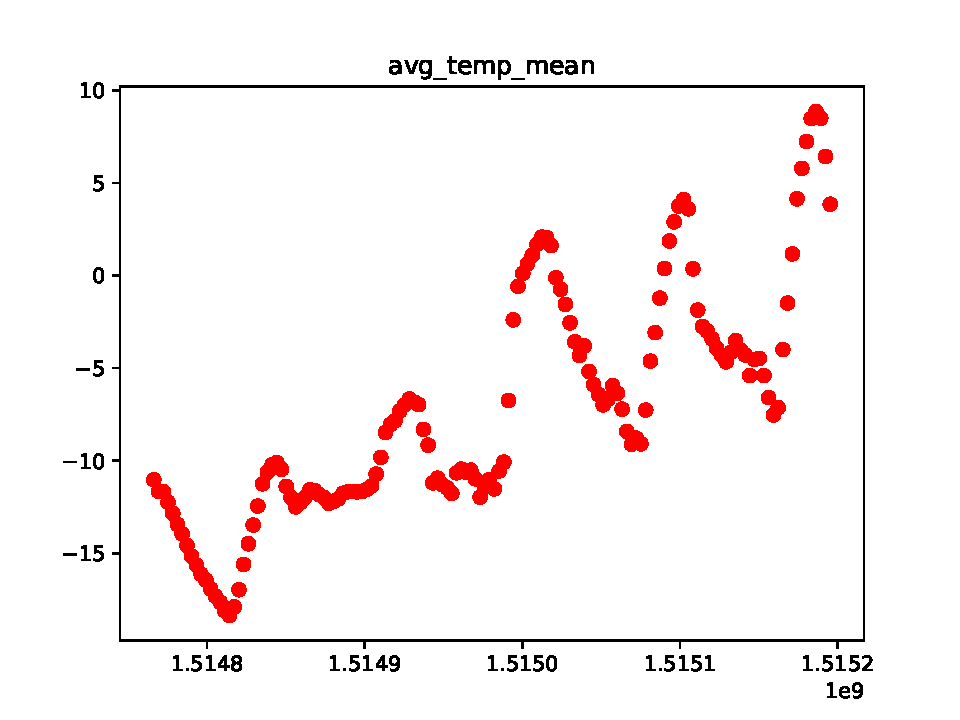
\includegraphics[width=0.6\textwidth]{../plots/avg_temp_mean.pdf}
    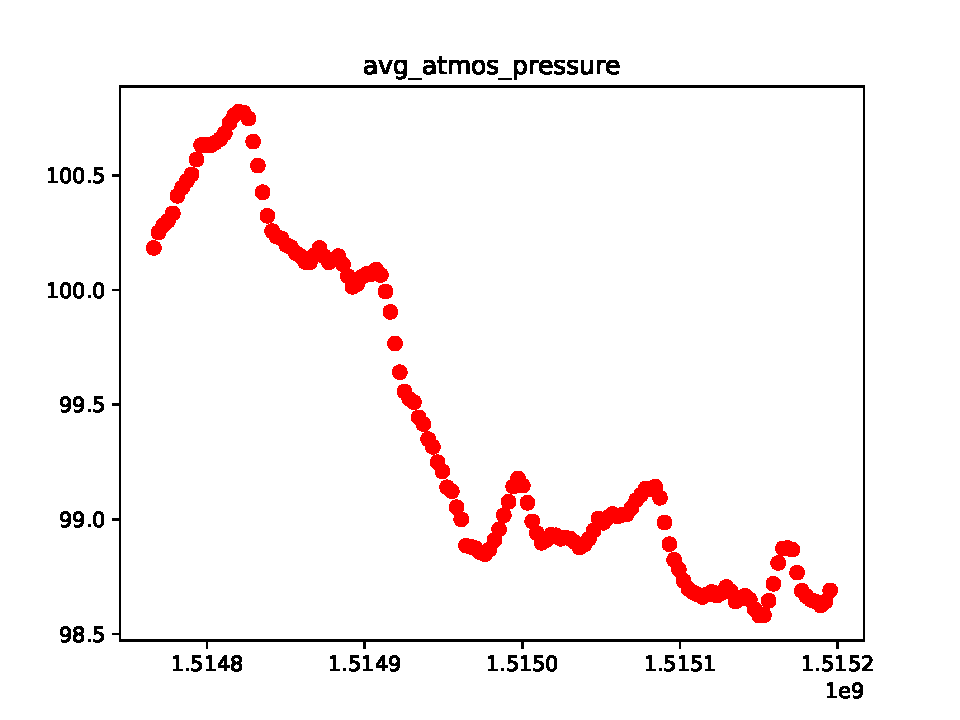
\includegraphics[width=0.6\textwidth]{../plots/avg_atmos_pressure.pdf}
    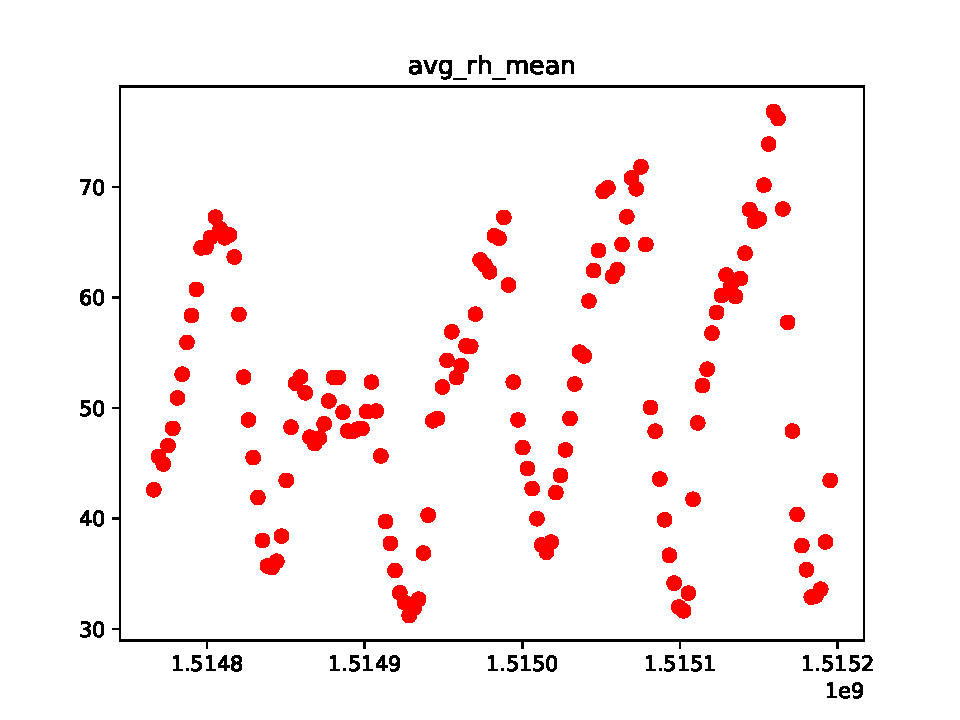
\includegraphics[width=0.6\textwidth]{../plots/avg_rh_mean.pdf}
    \caption{Time series of the average of mean temperature, mean relative humidity and atmospheric pressure as a function of time.}
\end{figure}

\section{Part 2: Clustering of data}

\subsection{$k$-means algorithm}
The goal here is to determine how the data are clustered.
The features we will use to find these clusters are the average temperature, atmospheric pressure and relative humidity and the derivatives of these quantities.
The clusters locations are determined using a $k$-means clustering algorithm that works in 2 steps that are repeated until convergence.
Given a number of cluster to find and a initial guess of the clusters centers, it first assigns all the data points to a cluster by determining the closest cluster center to each datapoint.
Then it calculates the average position of the obtained cluster.

Here I have used the scipy clustering package\footnote{\href{https://docs.scipy.org/doc/scipy/reference/cluster.vq.html}{Scipy clustering package}}.
Figure \ref{} shows the distance between the datapoints and each cluster center for various numbers of clusters.

\begin{figure}
    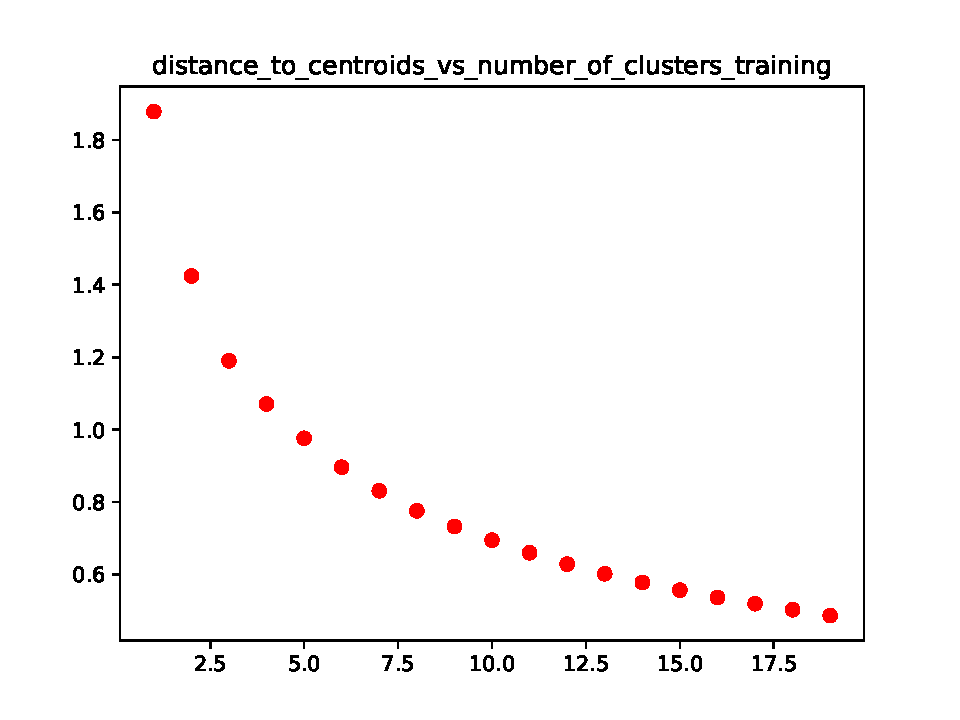
\includegraphics[width=0.45\textwidth]{../plots/distance_to_centroids_vs_number_of_clusters_training.pdf}
    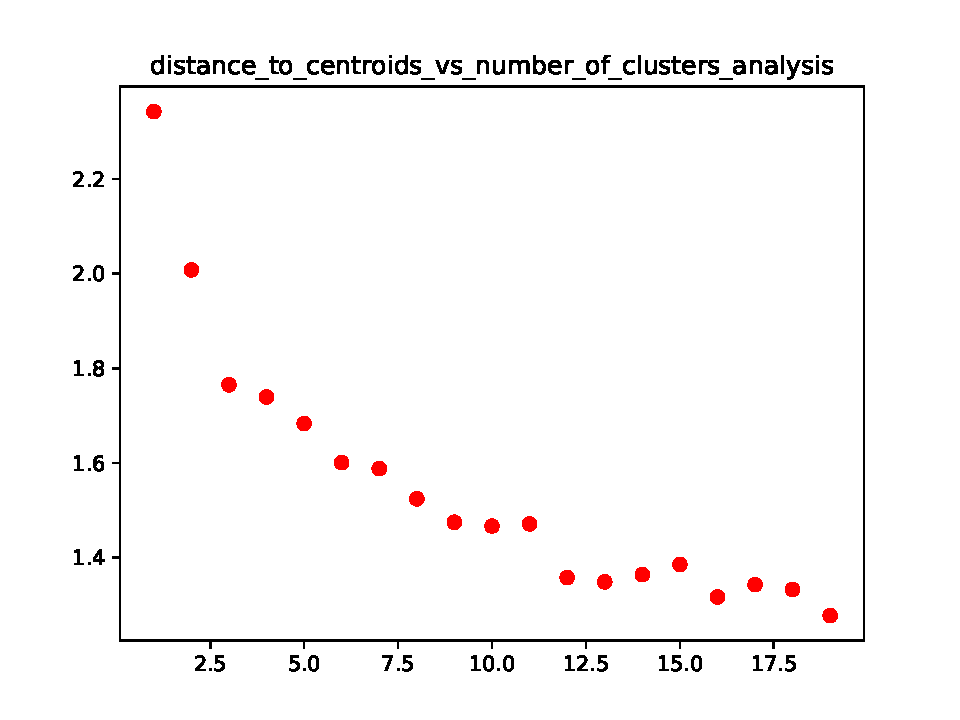
\includegraphics[width=0.45\textwidth]{../plots/distance_to_centroids_vs_number_of_clusters_analysis.pdf}
    \caption{Distance to the cluster centers as a function of the number of clusters: the plot on the right corresponds to the training dataset and the right to the testing dataset.}
\end{figure}




\subsection{Determination of the optimal number of clusters} 



\end{document}  

